% \chapter{Introduction}
\label{part:intro}

\tb{Clearly more on floation etc... ask for picture }
\section{Industrial challenges} 
Sedimentation of particles falling or rising under the action of gravity through a fluid is frequently used in a variety of industrial and natural processes, such as food processing, cosmetics, petroleum production, and environmental remediation. 
It is an efficient way to separate solid particles or droplets from the surrounded fluid. 
The clarification of waste water makes use of such a physics, the particles or droplets rise up due to buoyancy forces, afterward they are ejected from the mixture.
Even through numerous experimental and theoretical studies have been conducted on this topic, models are still very restricted and show a significant lack of accuracy. 
In the Perspective of reducing the cost and the environmental impacts of energy processes involving multiphase flows, IFP Energies Nouvelles and public funds, supply finance for the theoretical as well as for experimental research on multiphase flows.
Therefore, this thesis focus on the theoretical and numerical modeling of buoyant emulsion in the context of water waste treatment.  


\section{A multiscale problem} 
The Liquid /Liquid multiphase flows often involve multiscale physical phenomenons. 
Indeed, at the scale of the vessel we can consider the mixture as a homogeneous phase.
The physical properties and the hydrodynamics of the mixture, will depend on the microscale properties and the phases' interactions.
In the context of droplets those interactions are of two kinds. 
The first one is the hydrodynamical interactions between the dispersed phase and continuous phase.
Here, the scale of interest is the droplet scale.
The second type of interaction come from the van der Walls forces which act at the molecular scale. 
Then, we can already identify $3$ scales in this problem.
The scale of the bulk, or the vessel, where the medium seems homogeneous. 
The scale of the droplets, where hydrodynamic forces drive the flow. 
And finally, the molecular scale or the interface scale, where the chemical interaction drive the motions. 
Note that the chemical interactions also involve surfactant which won't be treated in this thesis. 

The link between the vessel's scale and the droplets' scale is usually made using averaged technics. 
It consists in averaging the constitutive equations, that drives the physics at the drop scale, to the reactor scale. 
For isothermal Newtonian flow we generally use the averaged Navier-Stokes equations \citep{jackson1997locally}. 
When we consider specific types of particles or fluid, we need to apply some changes to these equations. 
These averaged equations regardless of the hypothesis taken, involve what we call closure terms.
Those closures are the mathematical expression of the nature of the microstructure.
As an example the averaged drag force on the particles, the velocity fluctuations and the averaged torque and higher moments are closures terms. 
To solve those equations one needs a precise expression of the closure terms. 
Another problem tackled by averaged equations is the modeling of the local size distribution of the droplets. 
The distribution of size can be affected through migration of particles that have different rising velocity as a consequence of their size, and through coalescence and break up of the droplets. 
Note that the particle size distribution is of a major importance as the drag force and the other closure terms depends on it. 
Then, the most challenging part of this problem is not to solve the averaged equations, but rather to find empirical or theoretical closures. 
Regarding the link between the molecular scale and the upper scales, it is done through the modeling of chemical interactions.
Indeed, while the droplets are in contact chemical interaction influence greatly the probability of coalescence and therefore the coalesce rate. 
As a consequence it changes the drops size distribution too.

\section{Non-exhaustive authors cartography of particles suspension dynamics} 
\begin{figure}[h!]
    \begin{tikzpicture}[thick, scale=1, every node/.style={scale=0.5}]
        \node (img) at (0,0){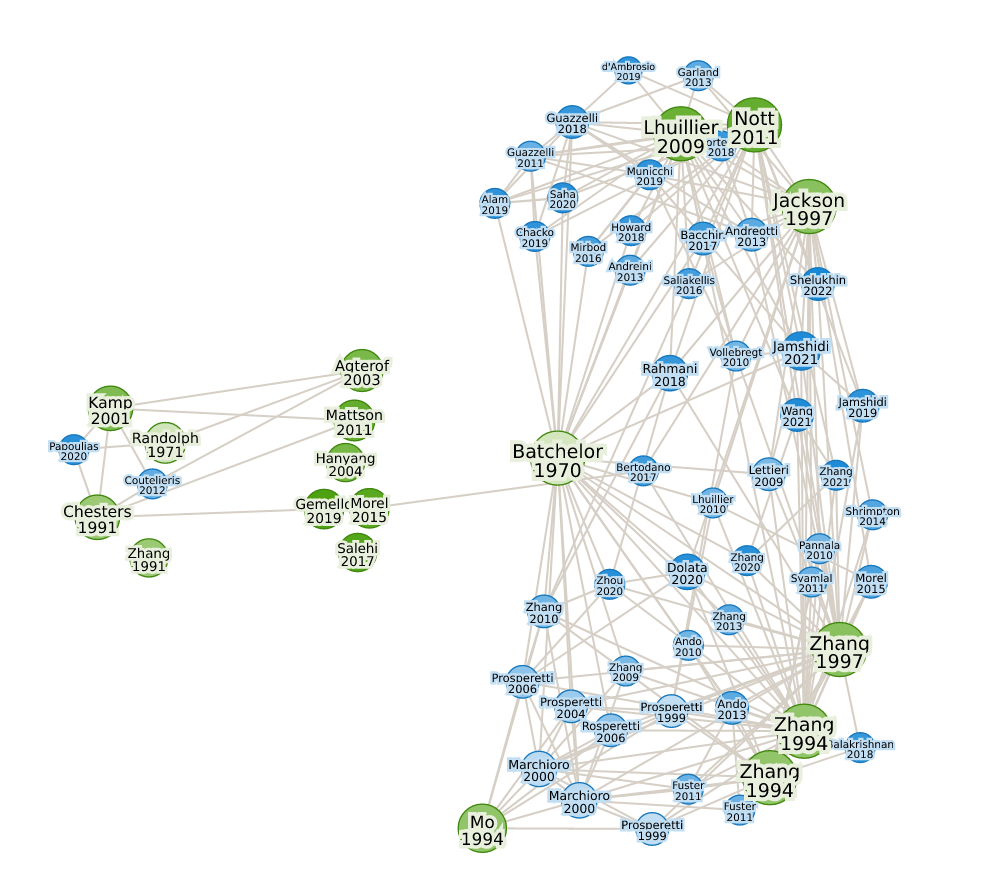
\includegraphics[width=2\textwidth]{Bib/graph70_paperGraph_network.png}};
        \draw[dashed,very thick](-2,-0.5)ellipse(1 and 2.5);
        \draw[dashed,very thick](-5,-0.5)ellipse(1.5 and 2.5);
        \draw[dashed,very thick](4,4)ellipse(2 and 1.5);
        \draw[dashed,very thick](4.5,-4)ellipse(1.5 and 2);
        \draw[dashed,very thick](4,5)node[above,very thick]{\Large$\bm{(III)}$};
        \draw[dashed,very thick](6,-5)node[right,very thick]{\Large$\bm{(II)}$};
        \draw[dashed,very thick](-6.5,2)node[above,very thick]{\Large$\bm{(I)}$};
        \draw[dashed,very thick](-1.3,1.75)node[above,very thick]{\Large$\bm{(IV)}$};
        % \draw[<->](com2.north)--(com3.south)node[midway]{Equivalent};
    \end{tikzpicture}
    \caption{Non-exhaustive cartography of the different publications on population balance models and averaged equations. The articles are represented by the name of the first author. The lines between each article mean that both articles cited each other.}
    \label{fig:carte}
\end{figure}
\ref{fig:carte} summarize the main area related to the theoretical modeling of emulsion through the averaged technics. 
The $\bm{(I)}$ field correspond to the modeling of coalescence and break up phenomenon in a drop or bubbles suspension.
It includes the Population Balance Model (PBM) theory.  
But also the modeling of the film drainage when two drops nearly coalesce. 
Indeed, \citet{randolph2012theory} introduced the first population balance models, at the origin it was designed  for Crystallizes. 
Then, \citet{chesters1991modelling} studied the hydrodynamical and chemical interaction of a pair of droplets leading to coalesce.
And finally, we can observe the first model of PBM including coalescence for a population of droplets \citep{KAMP20011363}.  
The $\bm{(II)}$ and $\bm{(III)}$ area are the authors who studied the averaged equations.
Most of them considered mono-dispersed suspension, therefore the PBE is not involved.
Rather they focused on closing the averaged equations theoretically. 
We consider two district formalism, the one represented here by the main article, \citet{jackson1997locally} and the other by \citet{zhang1994averaged}.
The first one makes use of volume average method and the second one of ensemble average method (those methods will be discussed in \ref{chap:avg}).
To model a poly-disperse suspension of particles (either solid, bubbles or droplet) one has to links the two former theories together, \citep{morel2015mathematical}. 
However, the current state of the art regarding droplets suspension is incomplete.
Therefore, in \ref{chap:avg}, after an entire review of the bibliography, we carry out the derivation of a generalized hybrid model for droplets particles. 
We will see that each of the terms of the averaged equations have a well-defined physical sense related to the nature of the particular phase. 
Then, we address the problematic of the identification of the essential closure terms, and evaluate their relative error while neglecting specific terms. 
Then, in \ref{chap:DNS} we tackle the problematic of the finding of closure terms through Direct Numerical Simulation (DNS).
After identifying the related investigation in the literature, we present our own model and a glimpse of our results in \ref{chap:mono-disperse}. 

\tb{introduce the main equations}